\documentclass{article}

\usepackage{tikz}
\usepackage[inner=0.5cm,outer=0.5cm,top=1cm,bottom=0.5cm]{geometry}

\pagestyle{empty}
\begin{document}
\thispagestyle{empty}

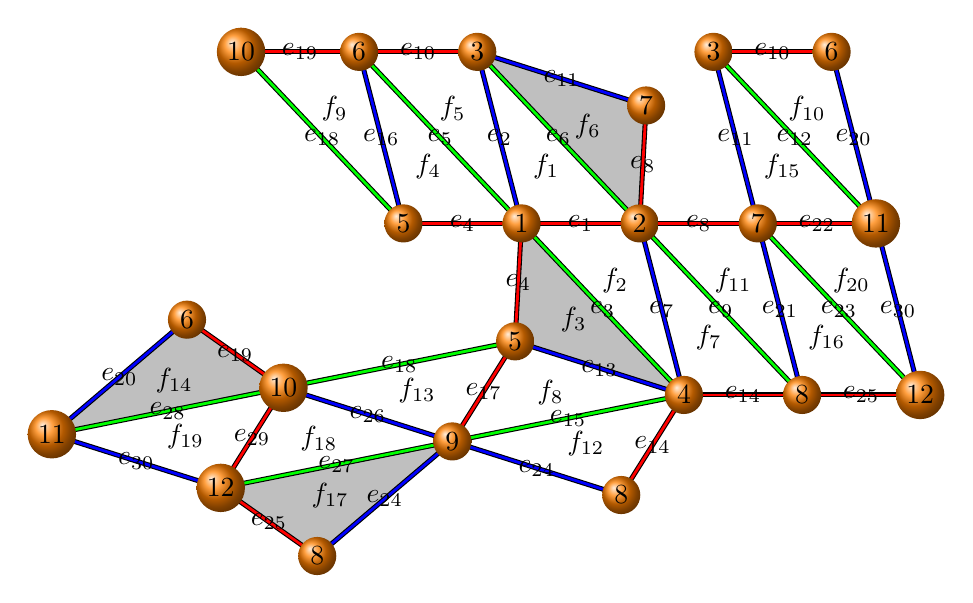
\begin{tikzpicture}[scale=3/4]
\coordinate (V1_1) at (0, 0);
\coordinate (V2_1) at (2, 0);
\coordinate (V3_1) at (-0.75, 2.904737509655563);
\coordinate (V3_2) at (3.25, 2.904737509655563);
\coordinate (V4_1) at (2.75, -2.904737509655563);
\coordinate (V5_1) at (-0.109375, -1.997007037888199);
\coordinate (V5_2) at (-2, 3.33066907387547e-16);
\coordinate (V6_1) at (-2.75, 2.904737509655563);
\coordinate (V6_2) at (5.25, 2.904737509655562);
\coordinate (V6_3) at (-5.6650390625, -1.630132638882223);
\coordinate (V7_1) at (2.109375, 1.997007037888199);
\coordinate (V7_2) at (4, -3.33066907387547e-16);
\coordinate (V8_1) at (4.75, -2.904737509655563);
\coordinate (V8_2) at (1.6875, -4.599167723621307);
\coordinate (V8_3) at (-3.4599609375, -5.631711135256683);
\coordinate (V9_1) at (-1.171875, -3.691437251853944);
\coordinate (V10_1) at (-4.75, 2.904737509655564);
\coordinate (V10_2) at (-4.03125, -2.783706780086581);
\coordinate (V11_1) at (6, -6.661338147750939e-16);
\coordinate (V11_2) at (-7.953125000000001, -3.570406522284963);
\coordinate (V12_1) at (6.75, -2.904737509655564);
\coordinate (V12_2) at (-5.09375, -4.478136994052326);


\fill[white] (V1_1) -- (V2_1) -- (V3_1) -- cycle;
\node (F1) at (0.4166666666666666, 0.9682458365518543) {$f_{1}$};
\fill[white] (V1_1) -- (V2_1) -- (V4_1) -- cycle;
\node (F2) at (1.583333333333333, -0.9682458365518543) {$f_{2}$};
\fill[lightgray] (V1_1) -- (V4_1) -- (V5_1) -- cycle;
\node (F3) at (0.8802083333333333, -1.633914849181254) {$f_{3}$};
\fill[white] (V1_1) -- (V5_2) -- (V6_1) -- cycle;
\node (F4) at (-1.583333333333333, 0.9682458365518546) {$f_{4}$};
\fill[white] (V1_1) -- (V3_1) -- (V6_1) -- cycle;
\node (F5) at (-1.166666666666667, 1.936491673103709) {$f_{5}$};
\fill[lightgray] (V2_1) -- (V3_1) -- (V7_1) -- cycle;
\node (F6) at (1.119791666666667, 1.633914849181254) {$f_{6}$};
\fill[white] (V2_1) -- (V4_1) -- (V8_1) -- cycle;
\node (F7) at (3.166666666666667, -1.936491673103709) {$f_{7}$};
\fill[white] (V4_1) -- (V5_1) -- (V9_1) -- cycle;
\node (F8) at (0.4895833333333333, -2.864393933132569) {$f_{8}$};
\fill[white] (V5_2) -- (V6_1) -- (V10_1) -- cycle;
\node (F9) at (-3.166666666666667, 1.936491673103709) {$f_{9}$};
\fill[white] (V3_2) -- (V6_2) -- (V11_1) -- cycle;
\node (F10) at (4.833333333333333, 1.936491673103708) {$f_{10}$};
\fill[white] (V2_1) -- (V7_2) -- (V8_1) -- cycle;
\node (F11) at (3.583333333333333, -0.9682458365518546) {$f_{11}$};
\fill[white] (V4_1) -- (V8_2) -- (V9_1) -- cycle;
\node (F12) at (1.088541666666667, -3.731780828376938) {$f_{12}$};
\fill[white] (V5_1) -- (V9_1) -- (V10_2) -- cycle;
\node (F13) at (-1.770833333333333, -2.824050356609574) {$f_{13}$};
\fill[lightgray] (V6_3) -- (V10_2) -- (V11_2) -- cycle;
\node (F14) at (-5.883138020833333, -2.661415313751255) {$f_{14}$};
\fill[white] (V3_2) -- (V7_2) -- (V11_1) -- cycle;
\node (F15) at (4.416666666666666, 0.9682458365518537) {$f_{15}$};
\fill[white] (V7_2) -- (V8_1) -- (V12_1) -- cycle;
\node (F16) at (5.166666666666666, -1.936491673103709) {$f_{16}$};
\fill[lightgray] (V8_3) -- (V9_1) -- (V12_2) -- cycle;
\node (F17) at (-3.241861979166667, -4.600428460387651) {$f_{17}$};
\fill[white] (V9_1) -- (V10_2) -- (V12_2) -- cycle;
\node (F18) at (-3.432291666666667, -3.65109367533095) {$f_{18}$};
\fill[white] (V10_2) -- (V11_2) -- (V12_2) -- cycle;
\node (F19) at (-5.692708333333333, -3.610750098807956) {$f_{19}$};
\fill[white] (V7_2) -- (V11_1) -- (V12_1) -- cycle;
\node (F20) at (5.583333333333333, -0.9682458365518549) {$f_{20}$};


\tikzset{EdgeStyle/.style = {thin, double distance=1pt} }

\draw[ EdgeStyle, double=red] (V2_1) -- node { $e_{1}$ } (V1_1);
\draw[ EdgeStyle, double=blue] (V1_1) -- node { $e_{2}$ } (V3_1);
\draw[ EdgeStyle, double=green] (V4_1) -- node { $e_{3}$ } (V1_1);
\draw[ EdgeStyle, double=red] (V5_1) -- node { $e_{4}$ } (V1_1);
\draw[ EdgeStyle, double=red] (V1_1) -- node { $e_{4}$ } (V5_2);
\draw[ EdgeStyle, double=green] (V1_1) -- node { $e_{5}$ } (V6_1);
\draw[ EdgeStyle, double=green] (V3_1) -- node { $e_{6}$ } (V2_1);
\draw[ EdgeStyle, double=blue] (V2_1) -- node { $e_{7}$ } (V4_1);
\draw[ EdgeStyle, double=red] (V7_1) -- node { $e_{8}$ } (V2_1);
\draw[ EdgeStyle, double=red] (V2_1) -- node { $e_{8}$ } (V7_2);
\draw[ EdgeStyle, double=green] (V2_1) -- node { $e_{9}$ } (V8_1);
\draw[ EdgeStyle, double=red] (V6_1) -- node { $e_{10}$ } (V3_1);
\draw[ EdgeStyle, double=red] (V3_2) -- node { $e_{10}$ } (V6_2);
\draw[ EdgeStyle, double=blue] (V3_1) -- node { $e_{11}$ } (V7_1);
\draw[ EdgeStyle, double=blue] (V7_2) -- node { $e_{11}$ } (V3_2);
\draw[ EdgeStyle, double=green] (V3_2) -- node { $e_{12}$ } (V11_1);
\draw[ EdgeStyle, double=blue] (V4_1) -- node { $e_{13}$ } (V5_1);
\draw[ EdgeStyle, double=red] (V8_1) -- node { $e_{14}$ } (V4_1);
\draw[ EdgeStyle, double=red] (V4_1) -- node { $e_{14}$ } (V8_2);
\draw[ EdgeStyle, double=green] (V4_1) -- node { $e_{15}$ } (V9_1);
\draw[ EdgeStyle, double=blue] (V5_2) -- node { $e_{16}$ } (V6_1);
\draw[ EdgeStyle, double=red] (V9_1) -- node { $e_{17}$ } (V5_1);
\draw[ EdgeStyle, double=green] (V5_2) -- node { $e_{18}$ } (V10_1);
\draw[ EdgeStyle, double=green] (V10_2) -- node { $e_{18}$ } (V5_1);
\draw[ EdgeStyle, double=red] (V10_1) -- node { $e_{19}$ } (V6_1);
\draw[ EdgeStyle, double=red] (V6_3) -- node { $e_{19}$ } (V10_2);
\draw[ EdgeStyle, double=blue] (V6_2) -- node { $e_{20}$ } (V11_1);
\draw[ EdgeStyle, double=blue] (V11_2) -- node { $e_{20}$ } (V6_3);
\draw[ EdgeStyle, double=blue] (V7_2) -- node { $e_{21}$ } (V8_1);
\draw[ EdgeStyle, double=red] (V7_2) -- node { $e_{22}$ } (V11_1);
\draw[ EdgeStyle, double=green] (V7_2) -- node { $e_{23}$ } (V12_1);
\draw[ EdgeStyle, double=blue] (V8_2) -- node { $e_{24}$ } (V9_1);
\draw[ EdgeStyle, double=blue] (V9_1) -- node { $e_{24}$ } (V8_3);
\draw[ EdgeStyle, double=red] (V12_1) -- node { $e_{25}$ } (V8_1);
\draw[ EdgeStyle, double=red] (V8_3) -- node { $e_{25}$ } (V12_2);
\draw[ EdgeStyle, double=blue] (V9_1) -- node { $e_{26}$ } (V10_2);
\draw[ EdgeStyle, double=green] (V9_1) -- node { $e_{27}$ } (V12_2);
\draw[ EdgeStyle, double=green] (V11_2) -- node { $e_{28}$ } (V10_2);
\draw[ EdgeStyle, double=red] (V12_2) -- node { $e_{29}$ } (V10_2);
\draw[ EdgeStyle, double=blue] (V11_1) -- node { $e_{30}$ } (V12_1);
\draw[ EdgeStyle, double=blue] (V12_2) -- node { $e_{30}$ } (V11_2);



\tikzset{VertexStyle/.style = {
 shape = circle,
 ball color = orange,
 text = black,
 inner sep = 2pt,
 outer sep = 0pt,
 minimum size = 10pt} }

\node[VertexStyle] at (V1_1) {1};
\node[VertexStyle] at (V2_1) {2};
\node[VertexStyle] at (V3_1) {3};
\node[VertexStyle] at (V3_2) {3};
\node[VertexStyle] at (V4_1) {4};
\node[VertexStyle] at (V5_1) {5};
\node[VertexStyle] at (V5_2) {5};
\node[VertexStyle] at (V6_1) {6};
\node[VertexStyle] at (V6_2) {6};
\node[VertexStyle] at (V6_3) {6};
\node[VertexStyle] at (V7_1) {7};
\node[VertexStyle] at (V7_2) {7};
\node[VertexStyle] at (V8_1) {8};
\node[VertexStyle] at (V8_2) {8};
\node[VertexStyle] at (V8_3) {8};
\node[VertexStyle] at (V9_1) {9};
\node[VertexStyle] at (V10_1) {10};
\node[VertexStyle] at (V10_2) {10};
\node[VertexStyle] at (V11_1) {11};
\node[VertexStyle] at (V11_2) {11};
\node[VertexStyle] at (V12_1) {12};
\node[VertexStyle] at (V12_2) {12};

\end{tikzpicture}

\end{document} 
